\section{Zielsetzung}
\label{sec:Zielsetzung}
Ziel des Versuches ist es die Bewegung der Leitungselektronen näher zu beschreiben. Dazu werden verschiedene mikroskopische Parameter aus den
zwei durchgeführten Versuchen berechnet.

\section{Theoretische Grundlage}
\label{sec:Theorie}

\subsection{Der Hall-Effekt}
Als Hall-Effekt wird das Auftreten einer Spannung in einem Stromdurchflossenen Leiter quer zur Richtung des Stroms bezeichnet, wenn sich der Leiter in einem äußeren Magnetfeld befindet. Die Spannung quer zur Stromrichtung lässt sich durch die Lorentz-Kraft erklären. In Abbildung \eqref{fig:Hall-Effekt} ist der  schematische Aufbau zur Beobachtung des Hall-Effektes zu sehen.

\begin{figure}[H]
	\centering
	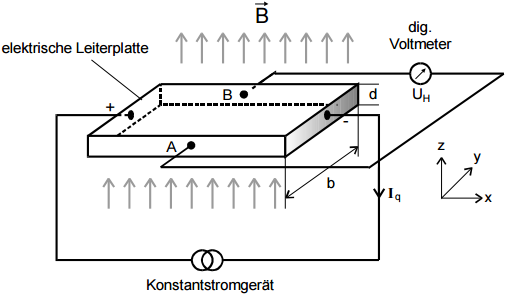
\includegraphics[height=7cm]{picture/Hall-Effekt.png}
	\caption{Schematischer Aufbau zur Beobachtung des Hall-Effektes. \cite[5]{sample}}
	\label{fig:Hall-Effekt}
\end{figure}

Am einfachsten ist der Leiter ein Quader der Breite $b$, der Länge $l$ und der Dicke $d$. Das Magnetfeld geht senkrecht durch die Fläche, welche von $b$ und $l$ aufgespannt wird. Der Strom fließt entlang der längsachse, wodurch auf die fließende Ladung die Lorentzkraft
\begin{equation}
	F_\text{L} = e_0\,\overline{v}_\text{D}\,B
\end{equation}
wirkt. Wobei $e_0$ für die Elementarladung, $v$ für die Geschwindigkeit der Elektronen und $B$ für die magnetische Flussdichte steht.


\subsection{Eigenschaft von Kristallen}


\subsection{Berechnung der elektrischen Leitfähigkeit eines Metalles}


\subsection{Fehlerrechnung}
Sämtliche Fehlerrechnungen werden mit Hilfe von Python 3.4.3 durchgeführt.
\subsubsection{Mittelwert}
Der Mittelwert einer Messreihe $x_\text{1}, ... ,x_\text{n}$ lässt sich durch die Formel
\begin{equation}
	\overline{x} = \frac{1}{N} \sum_{\text{k}=1}^\text{N} x_k
	\label{eqn:ave}
\end{equation}
berechnen. Die Standardabweichung des Mittelwertes beträgt
\begin{equation}
	\Delta \overline{x} = \sqrt{ \frac{1}{N(N-1)} \sum_{\text{k}=1}^\text{N} (x_\text{k} - \overline{x})^2}
	\label{eqn:std}
\end{equation}

\subsubsection{Gauß'sche Fehlerfortpflanzung}
Wenn $x_\text{1}, ..., x_\text{n}$ fehlerbehaftete Messgrößen im weiteren Verlauf benutzt werden, wird der neue Fehler $\Delta f$ mit Hilfe der Gaußschen Fehlerfortpflanzung angegeben.
\begin{equation}
	\Delta f = \sqrt{\sum_{\text{k}=1}^\text{N} \left( \frac{ \partial f}{\partial x_\text{k}} \right) ^2 \cdot (\Delta x_\text{k})^2}
	\label{eqn:var}
\end{equation}

\subsubsection{Lineare Regression}
Die Steigung und y-Achsenabschnitt einer Ausgleichsgeraden werden gegebenfalls mittels Linearen Regression berechnet.
\begin{equation}
	y = m \cdot x + b
	\label{eqn:reg}
\end{equation}
\begin{equation}
	m = \frac{ \overline{xy} - \overline{x} \overline{y} } {\overline{x^2} - \overline{x}^2}
	\label{eqn:reg_m}
\end{equation}
\begin{equation}
	b = \frac{ \overline{x^2}\overline{y} - \overline{x} \, \overline{xy}} { \overline{x^2} - \overline{x}^2}
	\label{eqn:reg_b}
\end{equation}
